\chapter{Introduction}

The field of autonomous driving agents has rapidly increased in modern car manufacturing. Current research topic rises the agents from parking or lane keeping assistant fully autonomous driving agents obeying the traffic rules and having the ability to react to the volatile environment in a reasonable way.

For that machine learning techniques have proven themselves as an essential part. But in order to fulfil the security standards and create a sophisticated agent it has to be trained on hundred-thousands of scenarios each having a large set of data attached, for example sensor and camera data.
The approach of \textit{Convolutional Neural Networks} (CNNs) have been proven to be powerful enough to handle such many training iterations with a huge number of input variables, while maintaining the large learning capacity. \cite{krizhevsky2012imagenet}

A CNN, as explained in \Cref{sec:CNN}, has a general structure, but can be altered to fit into the approach in various ways influencing the result. Therefore we introduce in \Cref{sec: Deep Learning Approaches} the three main approaches of using a CNN.

Further in \Cref{sec: DLL} we see that there is the need of specific languages for the design and implementation of such agents. Two languages will be discussed and compared based on their suitability regarding the \alexnet, stated in  \Cref{subsec: AlexNet}.

\section{Convolutional Neural Network (CNN)}\label{sec:CNN}

A CNN is a special class of deep feed-forward neural networks. On of the main design goals of a CNN is that they require a minimal amount of preprocessing. This is an important aspect, because they are often fed with images. Preprocessing high resolution images is very costly in terms of computational time. In the context of autonomous driving the time is even more crucial, since the driving agent needs to be able to react to spontaneous events.

Like most parts of neural networks, also the CNNs are inspired by biological processes. It is mainly based on the connectivity pattern of an animals visual cortex, where special neurons respond only to stimuli of their receptive field. Partially overlapping guarantees a complete coverage of the field of view. \cite{wiki:CNN}

Further CNNs make strong and mostly correct assumptions about the nature of images, like staionarity of statistics nad locality of pixel dependencies. This leads to fewer connections and parameters, compared to a normal feed-forward neural net with similar sized layers, and therefore reduces the time it takes to be trained, while being only slightly worse in their best-performance. \cite{krizhevsky2012imagenet}

\todo{\begin{enumerate}
\item how detailed? 
\item where starting?
\end{enumerate}}

\subsection{AlexNet} \label{subsec: AlexNet}

The \textit{\alexnet} is on of the best performing CNN architectures currently known. It is trained on the ImageNet subsets of \texttt{ILSVRC-2010} and \texttt{ILSVRC-2012}\footnote{Further information: http://www.image-net.org/challenges/LSVRC/} and became famous because of its result being way ahead of all other competitors.

A highly optimized GPU implementation of this architecture combined with innovative features is publicly available. Those features lead to improve performance and reduce training time.
An important note is that the original test is dated back to 2012 and therefore was used with an overall GPU memory of 6GB, with which training took abound six days. With modern hardware the training can be done faster, or the model can be trained much more. \cite{krizhevsky2012imagenet}

\todo{maybe calc the possible speed up based on ``Hardware for Machine Learning''}

\begin{figure}[ht]
	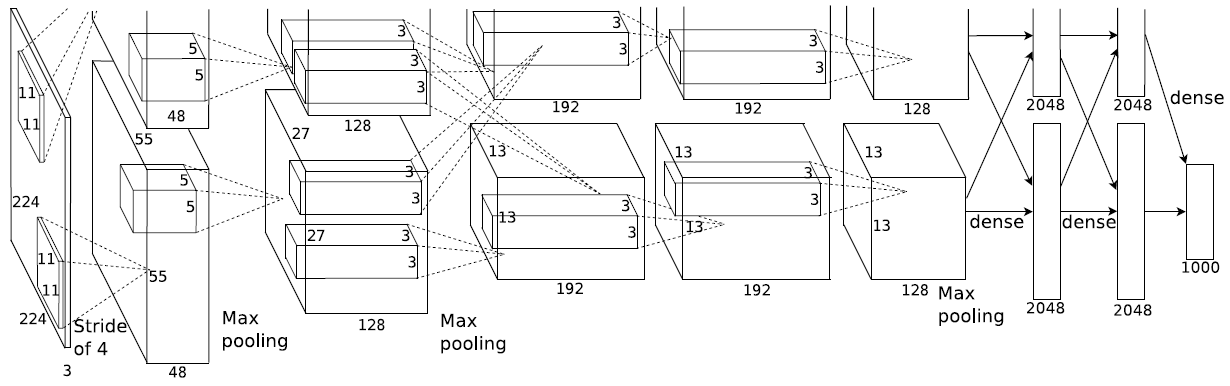
\includegraphics[scale = 0.5]{src/pic/AlexNet-structure.PNG}
	\caption{The \alexnet-architecture for two GPUs. It consists of 5 convolutional layers (at the beginning) and three fully-connected layers (at the end). The GPUs only communicate between two layers, but never within a layer.\cite{krizhevsky2012imagenet}}
	\label{pic: AlexNet}
	\todo{Vereinfachen der Zeichnung\\}
\end{figure}

\section{Available Deep Learning Approaches}\label{sec: Deep Learning Approaches}

There are various approaches of autonomous driving agents making a variety of assumptions and differ in numerous options. But they can be mostly categorized into two major groups of approaches: mediated perception approaches and behavior reflex approaches. \cite{chen2015deepdriving}

In this paper we further analyze a suggested third group, called direct perception, which can traced to \cite{gibson2014ecological} in the late 80's, but was sharply criticized by researchers of the other two groups, i.e. in \cite{ullman1980against}.

All these three groups differ in the way of interpreting the given sensor data and whether or not to create a some what bigger picture based on consequent data.

\subsection{Mediated Perception} \label{subsec: Mediated Perception}

The mediated perception approach is a multi-component continuous process. Every component recognizes specific aspects for driving. For example traffic signs, lanes, other cars. Those components are then combined into one single world state representing the cars surrounding based on the sensor data. \cite{KITTI}\\
These world states are 3D models of the current world. Cars are identified using a classifier and then often surrounded by a 3D bounding box. An example can be seen in \Cref{pic: 3D Bounding Box}. By comparing different frames generated one can estimate the speed and distance to those objects and derive an A.I. based precedence behavior. \cite{KITTI}\cite{chen2015deepdriving}

The often stated problems with such approaches are, that computing such a scene is costly in terms of computation time. Some information is irrelevant, redundant or even misleading due to inaccuracy of sensors. To perform a right turn the sensor information of the distance to a car left behind me is irrelevant, but becomes very important when taking a left turn.\\
Additionally many of the subtasks are still open research topics themselves. For example a reliable lane detection throughout various weather conditions or worse. Imagine a new road not having any drawn lines yet.\\
Also mediated perception approaches require very detailed information up front, like up-to-date maps.

The approach of mediated perception is a reasonable and very sturdy way of handling such a complex task, but has its drawbacks regarding computational time and additional knowledge.

\begin{figure}
	\centering
	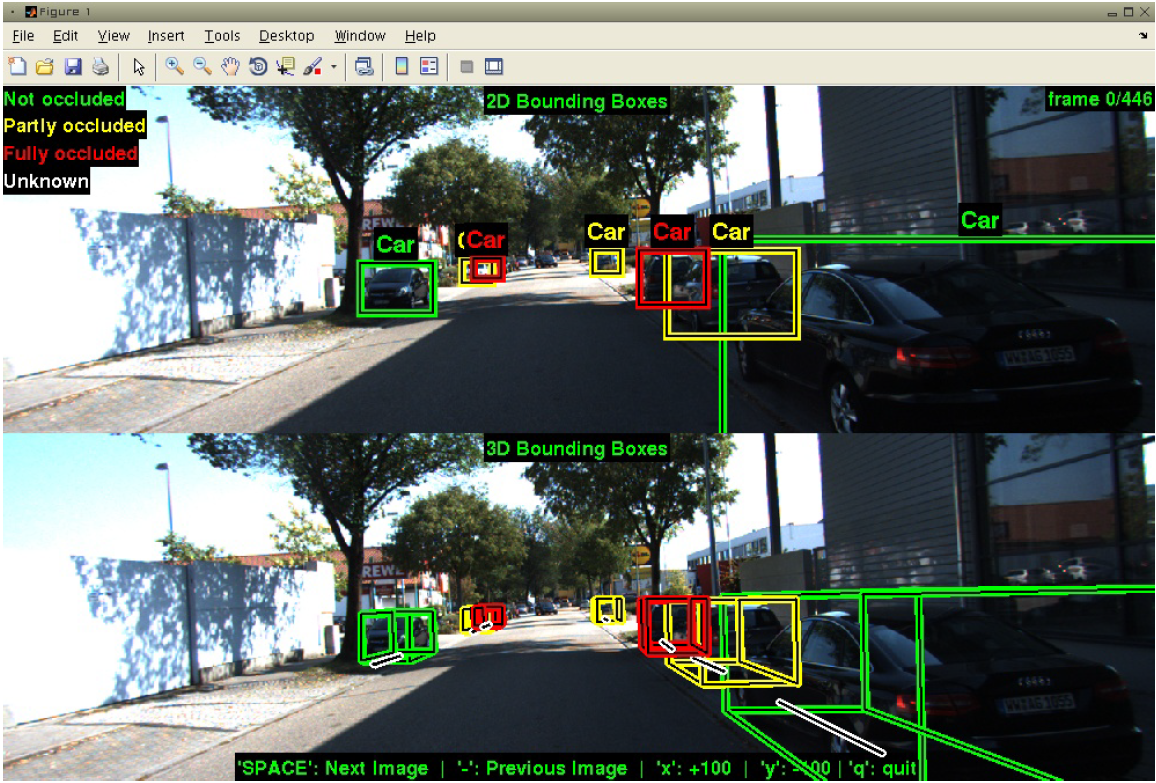
\includegraphics[scale=0.6]{src/pic/3D-boundingbox-example.png}
	\caption{An example of a scene using 3D bounding boxes. This image is taken from the MATLAB delvopment kit of \cite{KITTI}}
	\label{pic: 3D Bounding Box}
\end{figure}

\subsection{Behavior Reflex}\label{subsec: Behavior Reflex}

State the approach of a Behavior Reflex CNN

\subsection{Direct Perception}\label{subsec: Direct Perception}

State the approach of direct perception 

\section{Deep Learning Languages}\label{sec: DLL}
\todo{\begin{enumerate}
\item why need a language
\item what should it in general do?
\item state that different languages ex.
\end{enumerate}}

\subsection{CNNArch}\label{subsec: CNNArch}

general and some more in depth information about CNNArch based on \cite{CNNArch}

\subsection{MxNet}\label{subsec: MxNet}

general information from \cite{chen2015mxnet}

